\section{Overview of the SRAM Structure}
\label{sec:overview}


% address decode and mem array
The baseline SRAMs generated by OpenRAM have 1 read/write port as
shown in Figure~\ref{fig:sram_architecture}. The address is decoded
(Section~\ref{sec:addressdecoder}) into a one-hot set of word lines
(WL) which are driven by word line drivers
(Section~\ref{sec:wldriver}) over the bit-cell array
(Section~\ref{sec:bitcellarray}). To facilitate reads, the precharge
circuitry (Section~\ref{sec:precharge}) precharges the bitlines so
that the column mux (Section~\ref{sec:column_mux}) can select the
appropriate word which is then sensed by the sense amplifiers
(Section~\ref{sec:senseamp}).  Write drivers
(Section~\ref{sec:writedriver}) use the bidirectional nature of the
column mux to write the appropriate columns in a given memory row.

A representative layout of such a memory closely resembles the logical
representation and is shown in Figure~\ref{fig:layout_view}.  The
address and data flip-flops and control circuitry are not shown but
are detailed in Section~\ref{sec:control}.


\begin{figure}[htb]
\centering
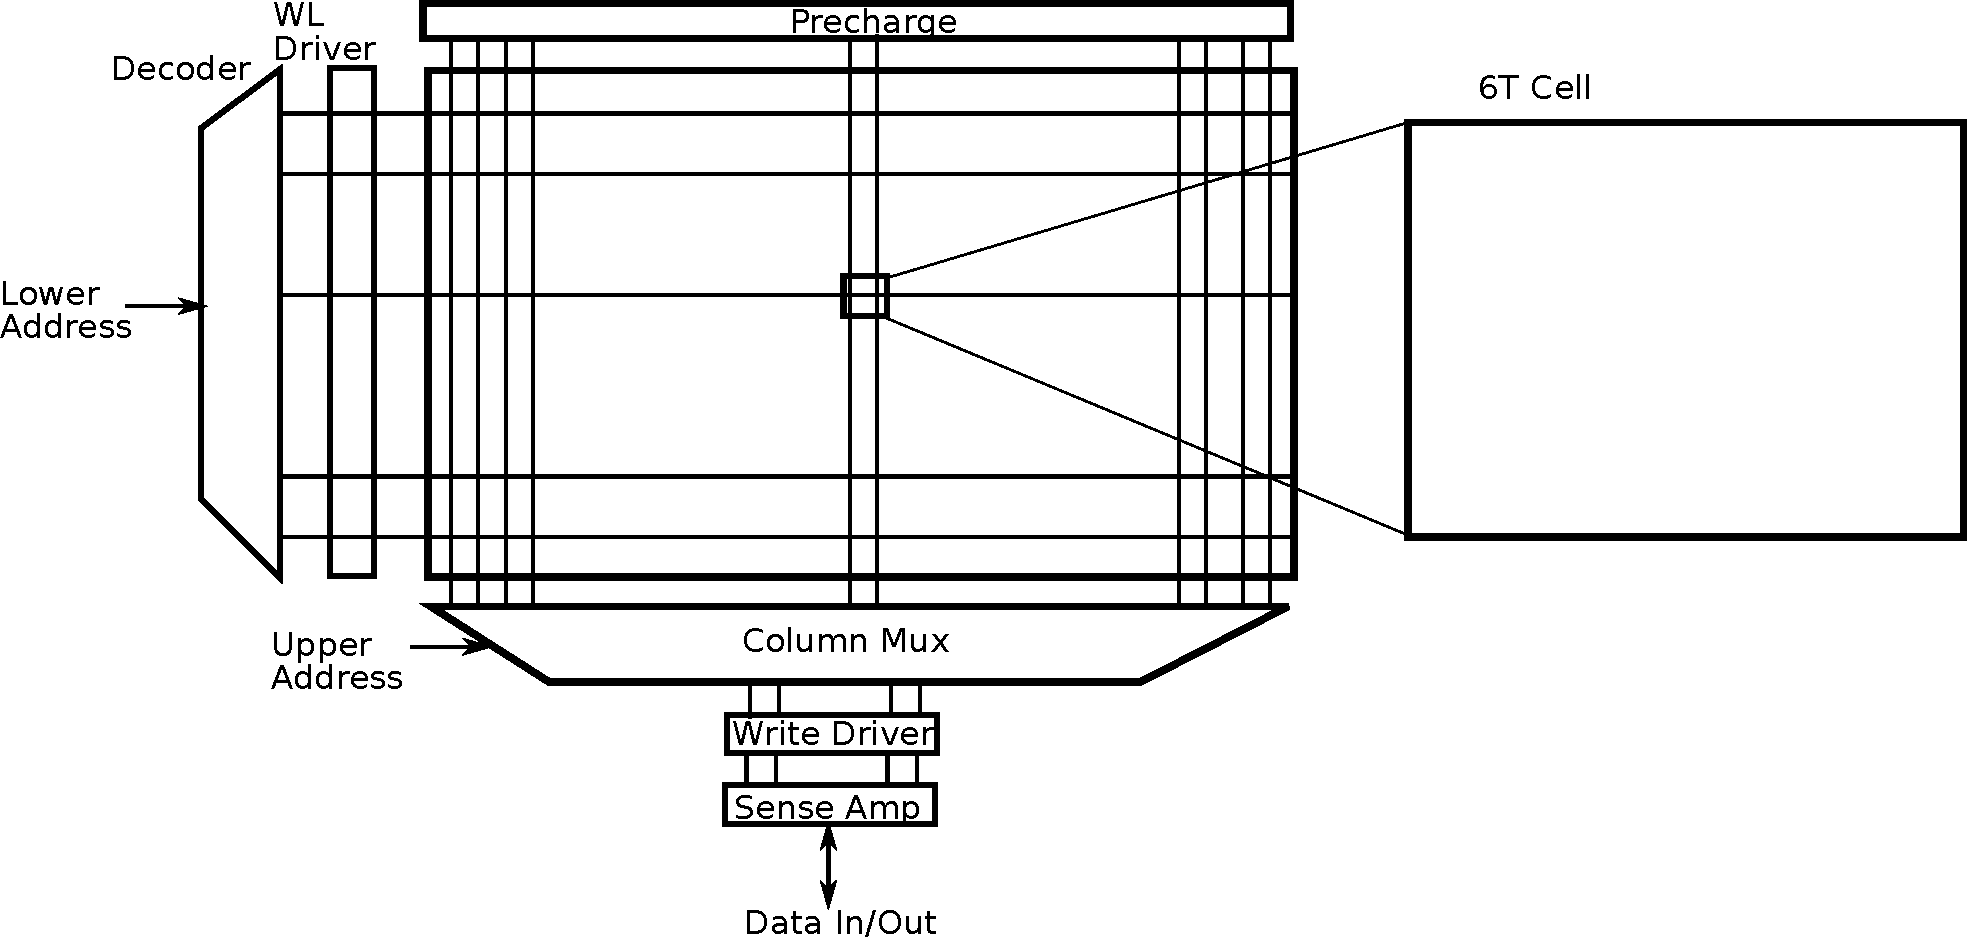
\includegraphics[width=10cm]{./figs/sram_overview.pdf}
\caption{Single Port SRAM Architecture}
\label{fig:sram_architecture}
\end{figure}


\begin{figure}[htb]
\centering
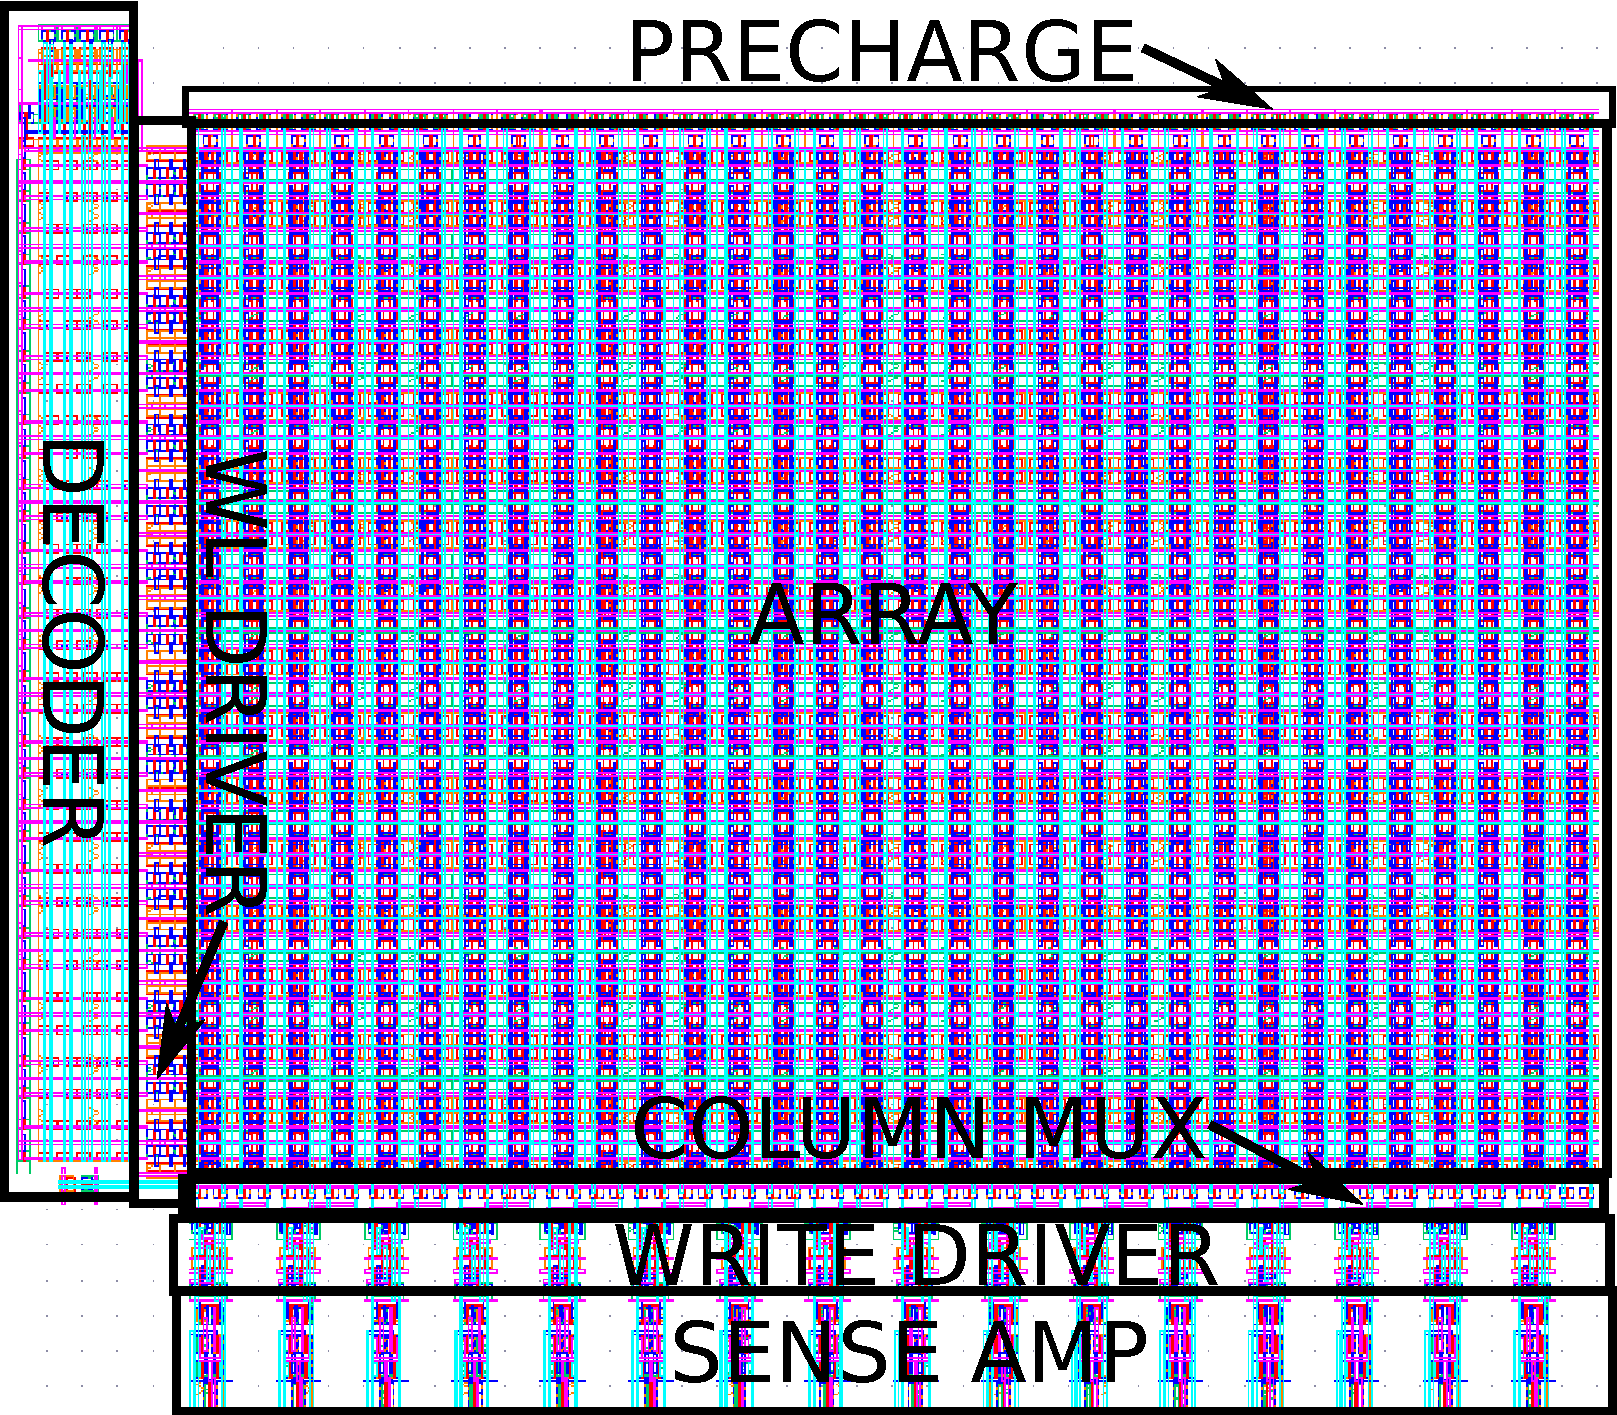
\includegraphics[width=6cm]{./figs/layout_view_1024_16_annotated.pdf}
\caption{1k SRAM with Two Columns and 16-bit Data}
\label{fig:layout_view}
\end{figure}



\subsection{Inputs/Outputs}
\label{sec:io}

The inputs to the SRAM are: 
\begin{itemize}
\setlength{\itemsep}{0pt}
\item clk - External Clock
\item CSb - Active-low Chip Select
\item WEb - Active-low Write Enable
\item OEb - Active-low Output Enable
\item ADDR\# - corresponds to the Address Bus input, labeled 0 to N-address bits.
\item DATA\# - corresponds to the bi-directional Data bus.
\end{itemize}

The outputs to the SRAM are: 
\begin{itemize}
\setlength{\itemsep}{0pt}
\item DATA\# - correspond to the bi-directional Data bus.
\end{itemize}


\subsection{Top-Level SRAM Module}
\label{sec:sram}

The \verb|sram| class in \verb|sram.py| is the top-level SRAM module.
This class handles the overall organization of the memory and the
input/output signals.  Based on the user inputs, the various bus and
array sizes are calculated and passed to the \verb|bank| module.
All other sub-modules access the value of sizes from \verb|bank|. 
The overall organization is depicted in
Figure~\ref{fig:sram_architecture}, discussion of the design data
structure is discussed in Section~\ref{sec:design} and the modules
contained in the top-level SRAM are detailed in
Section~\ref{sec:modules}.

When the user has specified the desired size (word size, total
number of words and number of banks) of the memory that is to be generated, 
the following parameters must be calculated. There are several constraints 
to be considered in this calculations:

(i) \verb|sram| can generate 1 bank, 2 banks or 4 banks.

(ii) The area of each bank should be as square as possible which is dependent on the area of a 6T cell.

(iii) There are several options for multiplexing (column-mux): 2-way, 4-way, 8-way  and none.


All of the top level routing is performed in the \verb|sram| class.

\fixme{More soon...}
